\documentclass{article}

%%% Fill details here (in the second brackets)
\newcommand{\name}{Hao Sun}     % Your name (First Last)
\newcommand{\wustlkey}{sun.hao}             % Your WUSTL Key
%%%



%%%%%%%%%%%%%%%%%%%%%% Formatting Stuff %%%%%%%%%%%%%%%%%%%%%%%%%%%
\usepackage{times}
\usepackage[T1]{fontenc}

\setlength{\parskip}{1em}\setlength{\parindent}{0pt}
\linespread{1.25}
\usepackage[margin=0.7in,top=1in]{geometry}\usepackage{fancyhdr}
\pagestyle{fancy}\lhead{\bf \name}\rhead{\bf \wustlkey}\cfoot{\thepage}
\newcommand{\info}{\clearpage \subsection*{Information}}

\newcommand{\solution}[1]{\clearpage \subsection*{Solution #1}}  % define a new command \solution without index number
\newcommand{\spart}[1]{\paragraph{(#1)}} 
%%%%%%%%%%%%%%%%%%%%%%%%%%%%%%%%%%%%%%%%%%%%%%%%%%%%%%%%%%%%%%%%%%%


%%% Add any more packages if you want to
\usepackage{amsmath,graphicx}


\begin{document}
%%%%% Main Body goes here

% Begin solution to every problem like this.
\solution{1}

\spart{a} 
	According to the slides in Lec2, the equation for $\epsilon$ is as follows:

\begin{equation}
  	\epsilon = g\sqrt{I^0}\epsilon_{1} + \sqrt{\left(g^2\sigma^2_{2a} + \sigma^2_{2b}\right)}\epsilon_{2}
\label{noise1}
\end{equation}

	So, the variation $\delta^2$ of $\epsilon$ is as follows:

\begin{align}
	\delta^2 &= \left(g\sqrt{I^0}\right)^2 + \left(\sqrt{\left(g^2\sigma^2_{2a} + \sigma^2_{2b}\right)}\right)^2\\
	&= g^2I^0 + g^2\sigma^2_{2a} + \sigma^2_{2b} 
	\label{variation1}
\end{align}

\spart{b} 
	Let $I^0 = \frac{I^0}{k}, g = gk$, we can get a new equation for new image I:

\begin{equation}
	I = gI^0 + gk\sqrt{\frac{I^0}{k}}\epsilon_{1} + \sqrt{\left(g^2k^2\sigma^2_{2a} + \sigma^2_{2b}\right)}\epsilon_{2}
\end{equation}

So, the zero-mean Gaussian noise $\epsilon$ is as follows:

\begin{equation}
	\epsilon = g\sqrt{kI^0}\epsilon_{1} + \sqrt{\left(g^2k^2\sigma^2_{2a} + \sigma^2_{2b}\right)}\epsilon_{2}
\end{equation}

	And its variation $\delta^2$ is:
\begin{equation}
	\delta^2 = g^2kI_{0}+ g^2k^2\sigma^2_{2a} + \sigma^2_{2b}
\end{equation}

\spart{c} 
	Because $I = \frac{\sum_{i=1}^{k}I_{i}}{k}$, and each $I_{i} = gI^0 + g\sqrt{kI^0}\epsilon_{1} + \sqrt{g^2k^2\sigma^2_{2a} + \sigma^2_{2b}}\epsilon_{2}$.\\
	So, the noise $\epsilon$ of I is:

\begin{equation}
	\epsilon = \frac{1}{k}\left(\epsilon1 + \epsilon2 + \cdots + \epsilon k \right)
\end{equation}

	The variation $\delta^2$ of $\epsilon$ is $\frac{1}{k^2}\left(\sigma^2_{1} + \sigma^2_{2} + \cdots + \sigma^2_{k}\right)$, and $\delta^2_{i} = g^2kI_{0} + g^2k^2\sigma^2_{2a} + \sigma^2_{2b}$. So $\delta^2$ is:

\begin{align}
	\delta^2 &= \frac{1}{k^2}k\left(g^2kI_{0} + g^2k^2\sigma^2_{2a} + \sigma^2_{2b}\right)\\
	&= g^2I_{0} + g^2k\sigma^2_{2a} + \frac{1}{k}\sigma^2_{2b}
	\label{variation2}
\end{align}

\spart{d} 
I think a single shot with exposure time $T$ is preferable. Because $k$ shots with exposure time $\frac{T}{k}$ will produce more noises based on equation of image $I$, even though variation $\delta^2$ of noise $\epsilon$ taking $k$ shots is similar to a single shot (it is determined by $k$), seen in (\ref{variation1}) and (\ref{variation2})
\begin{align}
	\epsilon = g\sqrt{I^0}\epsilon_{1} + \sqrt{g^2\sigma^2_{2a} + \sigma^2_{2b}}\epsilon_{2}\\
	\epsilon = g\sqrt{kI^0}\epsilon_{1} + \sqrt{g^2k^2\sigma^2_{2a} + \sigma^2_{2b}}\epsilon_{2}    (k shots)
\end{align}

\solution{2}

\begin{figure*}[h!]
  \centering
  	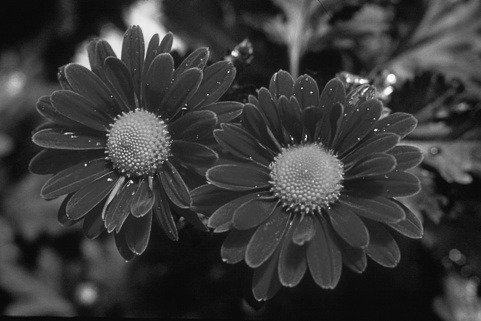
\includegraphics[height=25em]{code/inputs/p2_inp.png}
	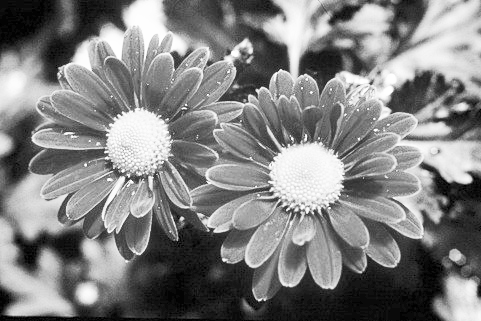
\includegraphics[height=25em]{code/outputs/prob2.png}
  \caption{Histogram equalization}
\end{figure*}

\solution{3}
\spart{a} Gradient magnitude
\begin{figure*}[h!]
  \centering
  	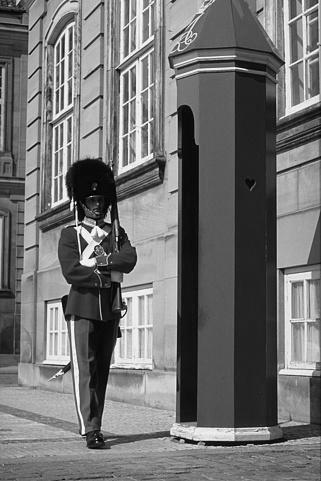
\includegraphics[height=35em]{code/inputs/p3_inp.png}
	
\includegraphics[height=35em]{code/outputs/prob3_a.png}
  \caption{gradient magnitudes}
\end{figure*}

\spart{b} NMS operation to optimize gradient magnitudes images

\begin{figure*}[h!]
  \centering
  	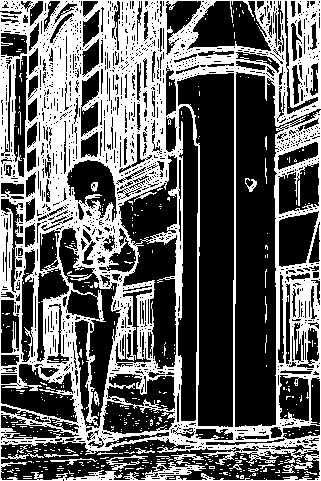
\includegraphics[height=20em]{code/outputs/prob3_b_0.png}
	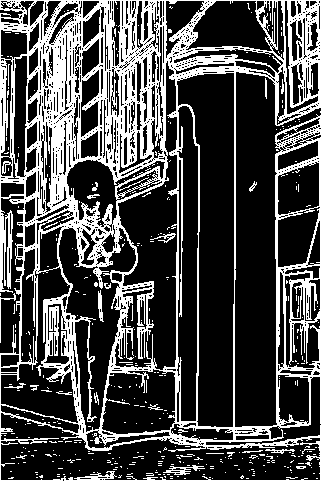
\includegraphics[height=20em]{code/outputs/prob3_b_1.png}
	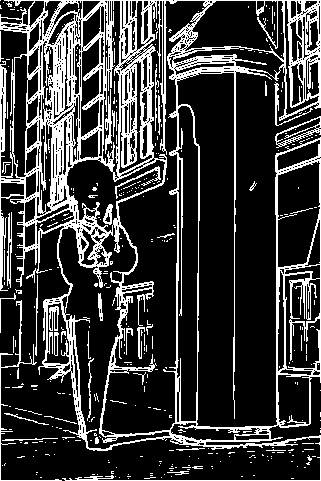
\includegraphics[height=20em]{code/outputs/prob3_b_2.png}
	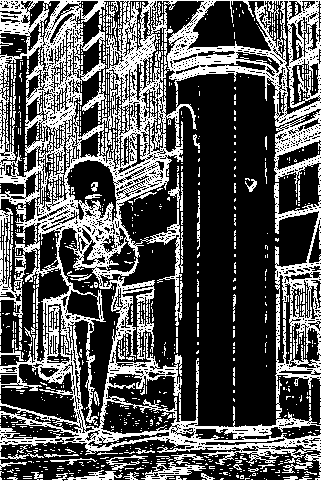
\includegraphics[height=20em]{code/outputs/prob3_b_nms0.png}
	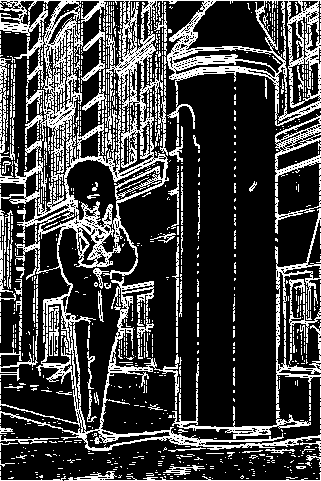
\includegraphics[height=20em]{code/outputs/prob3_b_nms1.png}
	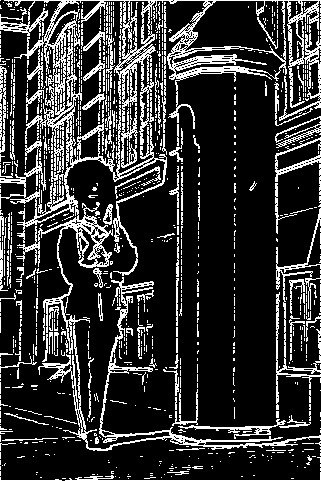
\includegraphics[height=20em]{code/outputs/prob3_b_nms2.png}
  \caption{NMS (lower level three pics)}
\end{figure*}

\solution{4} Bilateral Filtering

\begin{figure*}[h!]
  \centering
  	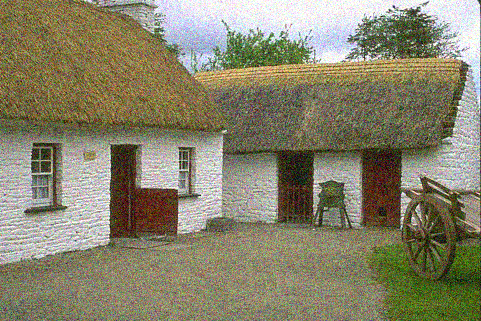
\includegraphics[height=20em]{code/inputs/p4_nz1.png}
  \caption{original image}
\end{figure*}

\begin{figure*}[h!]
  \centering
  	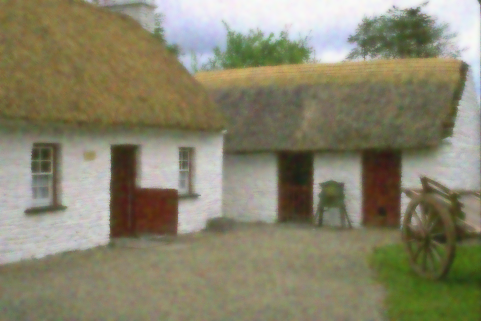
\includegraphics[height=16em]{code/outputs/prob4_1_a.png}
	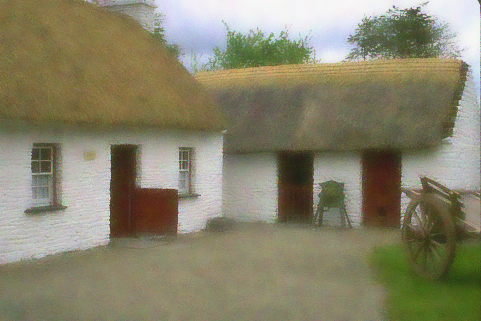
\includegraphics[height=16em]{code/outputs/prob4_1_b.png}
	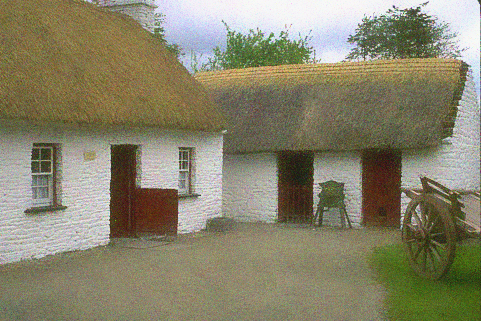
\includegraphics[height=16em]{code/outputs/prob4_1_c.png}
	 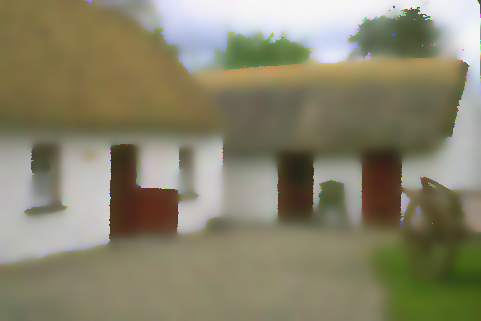
\includegraphics[height=16em]{code/outputs/prob4_1_rep.png}
  \caption{ $K=9, \sigma_s = 2,\sigma_I = 0.5$; $K=9, \sigma_s = 4,\sigma_I = 0.25$; 
  $K=9, \sigma_s = 16,\sigma_I = 0.125$;  repeat 8 times $K=9, \sigma_s = 2,\sigma_I = 0.125$}
\end{figure*}

\begin{figure*}[h!]
  \centering
  	 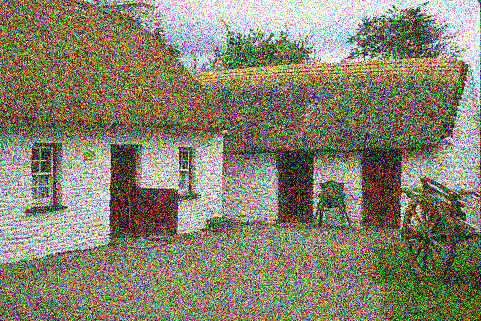
\includegraphics[height=20em]{code/inputs/p4_nz2.png}
	  \caption{Original image with more noise}
\end{figure*}

\begin{figure*}[h!]
  \centering
  	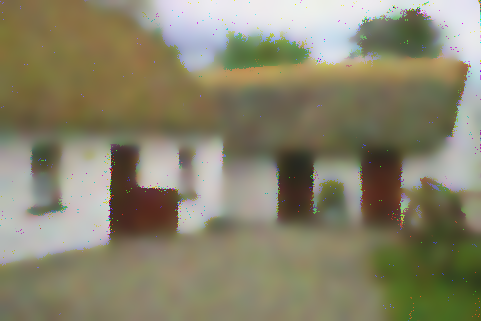
\includegraphics[height=20em]{code/outputs/prob4_2_rep.png}
  \caption{repeat 12 times $K=9, \sigma_s = 8,\sigma_I = 0.125$}
\end{figure*}

\solution{5}
\spart{a} 
 Because F[u,v] is central symmetry image. So we can store half of F[u,v] image.\\
 When both $W_x$, $H_x$ are even, the image size will be $W_x/2 * H_x$\\
 When both $W_x$, $H_x$ are odd, the image size will be $(\lfloor W_x/2 \rfloor + 1)*H_x$\\ 
 When $W_x$ is odd, $H_x$ is even, the image size will be $H_x/2*W_x$\\
 When $H_x$ is odd, $W_x$ is even, the image size will be $W_x/2*H_x$\\

\spart{b}  Convolution in the Fourier Domain:

\begin{figure*}[h!]
  \centering
  	
\includegraphics[height=20em]{code/outputs/prob5.png}
  \caption{Convolution in the Fourier Domain}
\end{figure*}

\solution{6}
\spart{a} Harr wavelet decomposition
\begin{figure*}[h!]
  \centering
  	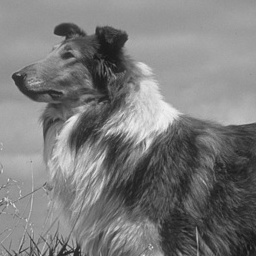
\includegraphics[height=20em]{code/inputs/p6_inp.png}
  \caption{Original image before Harr Wavelet Decompostion}
\end{figure*}

\begin{figure*}[h!]
  \centering
  	
\includegraphics[height=16em]{code/outputs/prob6a_1.png}
	
\includegraphics[height=16em]{code/outputs/prob6a_2.png}
	
\includegraphics[height=16em]{code/outputs/prob6a_3.png}
  \caption{Image after Harr Wavelet Decompostion}
\end{figure*}


\spart{b} Image reconstruction from Harr wavelet decomposition

\begin{figure*}[h!]
  \centering
  	
\includegraphics[height=18em]{code/outputs/prob6b.png}
	
\includegraphics[height=18em]{code/outputs/prob6b_0.png}
	
\includegraphics[height=18em]{code/outputs/prob6b_1.png}
	
\includegraphics[height=18em]{code/outputs/prob6b_2.png}
  \caption{Image reconstruct from Harr Wavelet Decompostion}
\end{figure*}





\info

This problem set took approximately 40 hours of effort.


I discussed this problem set with:
\begin{itemize}
\item Sijia Wang
\item Chunyuan Li
\item Likai Yan
\end{itemize}


% Note that you might have to escape some special symbols in URLS like \_
I also got hints from the following sources:
\begin{itemize}
\item Wikipedia article on matrix calculus at https://en.wikipedia.org/wiki/Matrix\_calculus
\item Read array operation from http://cn.mathworks.com/help/matlab/ref/circshift.html?s\_tid=gn\_loc\_drop
\item Read numpy tutorial from http://cs231n.github.io/python-numpy-tutorial/
\item Study complex number from https://www.khanacademy.org/math/algebra2/introduction-to-complex-numbers-algebra-2/the-complex-numbers-algebra-2/v/complex-number-intro
\item Get mathematical functions from https://docs.scipy.org/doc/numpy/reference/routines.math.html
\item Study how to use LaTeX from https://www.latex-tutorial.com/tutorials/
\item Study the process of Bilateral filter from http://blog.csdn.net/abcjennifer/article/details/7616663
\item Understand Fourier Transform from http://blog.jobbole.com/70549/
\item Study Fourier Transform in Imaging process from http://m.blog.csdn.net/abcjennifer/article/details/7622228
\end{itemize}

\end{document}
